\documentclass[11pt,
  oneside,openany,    % for one-sided printing and screens
  %draft              % enable to compile faster and test layout
]{scrreprt}

% Settings
\usepackage[table]{xcolor}
\usepackage[ngerman,english]{babel}
\usepackage[utf8]{inputenc}
\usepackage{geometry}
\usepackage{microtype}
\usepackage[all]{nowidow}
\usepackage{csquotes}
\usepackage{dsfont}

\usepackage[bsc,             % for Bachelor's Thesis titlepage
            %project,        % for Master's Project titlepage
            claim,iaik]{iaikthesis}
\addtokomafont{disposition}{\rmfamily}

% <INSERT YOUR CUSTOM MACROS AND PACKAGES HERE>
\usepackage{booktabs}
\usepackage{caption}
\usepackage{upgreek}
\usepackage[linesnumbered, ruled, lined, boxed]{algorithm2e}
\usepackage[skip=10pt plus1pt, indent=10pt]{parskip}
\usepackage{graphicx}
\usepackage{minted}
\RecustomVerbatimEnvironment{Verbatim}{BVerbatim}{}
\usemintedstyle{colorful}
\usepackage{tcolorbox}
\usepackage{multirow}
\newtcbox{\inlinecode}{on line, boxrule=0pt, boxsep=0pt, top=2pt, left=2pt, bottom=2pt, right=2pt, colback=gray!15, colframe=white, fontupper={\ttfamily \footnotesize}}
% source: https://tex.stackexchange.com/questions/2705/typesetting-column-vector

\newcommand{\gmidrule}{\arrayrulecolor{lightgray}\specialrule{\lightrulewidth}{0.4\aboverulesep}{0.6\belowrulesep}\arrayrulecolor{black}}

\newcount\colveccount
\newcommand*\colvec[1]{
        \global\colveccount#1
        \begin{pmatrix}
        \colvecnext
}
\def\colvecnext#1{
        #1
        \global\advance\colveccount-1
        \ifnum\colveccount>0
                \\
                \expandafter\colvecnext
        \else
                \end{pmatrix}
        \fi
}
% algorithm comment
\SetKwComment{Comment}{/* }{ */}
% floor cmd
\newcommand{\floor}[1]{\lfloor {#1} \rfloor}
\newcommand{\ceil}[1]{\lceil {#1} \rceil}

% Useful packages for complex content:
\usepackage{amsmath,amsfonts,amssymb} % typesetting math
\usepackage{centernot}
%\usepackage{tikz}                    % typesetting diagrams, figures, ...
%\usepackage{siunitx}                 % typesetting SI-units and formatted numbers
%\usepackage{listings}                % typesetting source code
%\usepackage{booktabs,multirow}       % utils for complex/beautiful tables
%\usepackage{subcaption}              % placing multiple subfigures in a figure

% Useful utils:
\usepackage{blindtext}                % insert dummy text for this template
%\usepackage{todonotes}               % add ToDo markers (\todo{...})
%\usepackage{xspace}                  % define macros that don't eat the following space (add \xspace at the end)
%\usepackage[section]{placeins}       % prevent figures from floating into the wrong section (\FloatBarrier)

% Bibliography, referencing, and indexing
\usepackage{csquotes}                 % typesetting \enquote{text in quotes} correctly
\usepackage[backend=biber,
            style=alphabetic,
            maxbibnames=20]{biblatex} % to generate the bibliography
\addbibresource{thesis.bib}           % name of the bib-file

\usepackage[hidelinks]{hyperref}      % clickable links (but hide color frames around links)
%\usepackage{cleveref}                % named references (\Cref{chap:introduction}, ...)

\usepackage[toc,acronym,style=long3col]{glossaries} % List of acronyms and symbols  (optional)
\makenoidxglossaries
%
\newacronym{aes}{AES}{Advanced Encryption Standard}
\newglossaryentry{xor}{name={\ensuremath{\oplus}}, sort=xor,
                       description={exclusive-or (\textsc{Xor})}}
% <INSERT YOUR GLOSSARY ENTRIES HERE (or \input{} a dedicated file) >



\begin{document}

%--- INSERT INFORMATION FOR TITLEPAGE ------------------------------------------

% Your name + previous academic degrees:
\thesisauthor{Bernhard Berg}

% Title of your thesis:
\thesistitle{Classic McEliece in Rust}

% Date of completion:
\thesisdate{June 2022}

% Supervisor:
\supervisortitle{Supervisors} % or Supervisor
\supervisor{%
  Lukas Prokop, Daniel Kales\\
  \smallskip

  Institute of Applied Information Processing and Communications\\
  Graz University of Technology
}

% Name of your degree programme according to your curriculum
%\curriculum{CurriculumName}
%\curriculum{Information and Computer Engineering}
%\curriculum{Computer Science}
\curriculum{Software Engineering and Management}



%--- FRONT MATTER --------------------------------------------------------------

\printthesistitle

\chapter*{Abstract}
The asymmetric McEliece cryptosystem, although previously unpopular in the cryptographic community due to its large key size, has become an exciting candidate in post-quantum cryptography because the hardness assumption of the underlying cipher remains unaffected by quantum computer attacks. In 2016 the NIST (National Institute of Standards and Technology) initiated the open post-quantum cryptography competition where the key-encapsulation mechanism classic McEliece is a round 3 candidate. The goal of this bachelor thesis is to understand the McEliece cryptosystem and port the classic McEliece implementation from the C programming language to the Rust programming language. Rust is a language that was developed with the focus on memory safety, specifically enabling safe low-level memory manipulation while at the same time offering multi-paradigm language features such as generics, pattern matching, iterators, and many more. In the course of this thesis, a Rust implementation of classic Mceliece was published as a crate (library) on the Rust community crate registry. The Rust implementation yields faster results than the C reference implementation in speed benchmarks.

\paragraph{Keywords:}
Post-quantum cryptography, Rust programming language, code-based cryptography, Classic McEliece, binary goppa codes

%\cleardoublepage
\tableofcontents  % optional



%--- MAIN CONTENT --------------------------------------------------------------
% begin equation starts equation block which gets incremental number annotated as text
% begin equation* <- start equation block without number annotation
\chapter{Introduction}
\label{chap:introduction}

In the current digitalized world, the field of cryptography represents a technical option to maintain a secure information exchange. Its purpose is to draft and verify protocols that ensure data integrity (no third-party modifications), confidentiality (no third-party inspection), and authenticity (the receiver of a message can verify the sender). The real-world applications range from payment systems in digital commerce to secure messenger applications for smartphones, where low-level cryptographic primitives enable a secure communication channel to avoid information leakage to potential adversaries.

In order to enable the security property of many cryptographic protocols, one-way functions are incorporated in these schemes which are comparatively feasible to compute in a forward direction independent on the input, however incredibly difficult to inverse a certain output to the desired input again~\cite{Kryptografie2016}.
\begin{gather*}
    \text{A generic function} \ f() \ \text{is defined as a one-way function if the following conditions hold:}\\
    a = f(b) \ \ \text{computationally feasible to calculate a from b}\\
    b = f^{-1}(a) \ \ \text{computationally infeasible to compute b from a}\\
\end{gather*}
In this context, the term computationally feasible is defined as that the function is computable in deterministic polynomial runtime where the polynomial degree determines the growth of the described algorithm. Such functions are considered practically solvable in the complexity class $P$ (polynomial).

A trapdoor function is a particular case of a one-way function where the same property holds that computation in the forward direction is feasible. However, calculating the inverse of a trapdoor function is only possible with the knowledge of the secret "trapdoor" information. Contrary to one-way functions, calculating the inverse of a trapdoor function recovers the complete input. For instance, additionally, the encryption randomness can be obtained~\cite{trapdoor}.

Up to date, two of the most essential one-way functions used in cryptographic schemes are the integer factorization problem (used in the RSA public-key cryptosystem) and the discrete logarithm problem, which is applied in public-key cryptographic systems using elliptic curves and Diffie–Hellman key exchange~\cite{Kryptografie2016}.

It is essential not to assume that one-way functions remain indefinitely secure. Their security is only valid as long as no method efficiently solves the backward direction. In 1997 Peter W. Shor published efficient randomized algorithms which solve the integer factorization and the discrete logarithm problems, given a theoretically powerful quantum computer on which these algorithms are exectued~\cite{pshor1997}. The implications of these findings triggered the scientific community to think about the future of cryptography once quantum computers are built, capable of fast and reliable integer factorization. 

\section{Post-quantum cryptography}

The objective of post-quantum cryptography is to design protocols that are, to the best of our knowledge, secure against targeted quantum-computer attacks, in addition to being secure against classical adversarial approaches. In order to concentrate efforts on reaching this goal, the NIST (The National Insitute of Standards and Technology of the United States) organized an open competition for quantum-resistant public-key encryption, key-establishment, and digital signature algorithms in December 2016~\cite{nistPQCcompetitionAnnounce}. 
The current scientific advancements in post-quantum cryptography can be categorized in the following research areas: Lattice-based cryptography, Hash-based cryptography, Multivariate cryptography, Isogeny-based cryptography, and Code-based cryptography.

In 1978 a public-key cryptosystem based on random binary irreducible error-correcting goppa codes was published by Robert J. McEliece~\cite{robertmceliece}. The one-way functionality of the McEliece cryptosystem relies on the decoding problem of binary goppa codes. Over the years, multiple cryptanalytic attacks have been published on the McEliece cryptosystem. However, with adjusted system parameters, the scheme remains unbroken as of today and has been shown to resist quantum attacks~\cite{engelbertOverbeckSchmidt, bernsteinLange, DinhMooreRussell}. Thus the security confidence in this cryptographic protocol is high, and since it does not rely on a problem currently known to be broken by quantum computers, the coding-based McEliece cryptosystem is a suitable candidate for post-quantum cryptography. The NIST competition lists "Classic McEliece" as a current round 3 finalist for public-key encryption and key-establishment algorithms~\cite{nistRound2summary}. Classic McEliece is a key encapsulation mechanism (KEM) built on a variant of the McEliece public-key encryption scheme using binary goppa codes.
The authors of the round 3 submission have provided a public package containing an implementation of Classic McEliece in the programming language C with detailed supporting information~\cite{classicMcElieceSubmission3}. While sophisticated research is being done on upcoming post-quantum cryptographic frameworks, another critical problem represents security vulnerabilities in cryptographic libraries. The security of internet network communication relies on cryptographic implementations, and concealed exploits in such code pose a considerable threat. The comprehensive review by Blessing et al~\cite{youShouldNtRollOwnCrypto} shows that $37.2\%$ of vulnerabilities originate from memory-safety issues in contrast to $27.2\%$ being cryptographic errors. The programming language Rust attempts to provide a solution to various memory safety bugs (for instance, buffer-overflows, use-after-free) by introducing strict semantic compiler checks for such errors. Rust has been created at Mozilla Research to maintain fast runtime performance while at the same time offering safe memory and type manipulations. The core of safe memory handling in Rust is its concept of ownership. Each memory resource where read/write manipulations are desired must have a reference variable flagged as its "owner". Only with this special entitlement the memory operations are allowed to proceed. With this concept, Rust aims to prevent dangling references which have not been invalidated, such as freed pointers in C/C++, which could still be accessed~\cite{RustBelt, memsafetyHui}.

\section{Contributions}
A pure Rust implementation has been carried out in the course of this thesis, which provides the Classic McEliece KEM to the Rust programming language. 
In the background section, basic concepts of linear algebra, coding theory, KEM, and the McEliece cryptosystem are explained. Furthermore, a chapter with more details on Rust's memory safety concepts is provided. In the implementation \& evaluation section, the experienced challenges of porting C language code to Rust, benchmark comparison, and differences in the implementations will be explained. 

The source code is released on Github:

\url{https://github.com/Colfenor/classic-mceliece-rust}

and as a crate on Rust crates.io registry:

\url{https://crates.io/crates/classic-mceliece-rust}


% You may want to keep your chapters in separate files ('chapterfilename.tex')
% and include them here using either
%\input{chapterfilename.tex}   or   \include{chapterfilename}
\chapter{Background}
\label{chap:background}

\newcommand\spacebetweenparandheader{\vspace{20pt}}

 A quick introduction to linear codes and a few basic definitions of linear algebra and coding theory are given first as fundamentals to understand the McEliece cryptosystem. Furthermore, it is assumed that the reader is acquainted with finite fields $\mathbb{F}_{q}$, the matrix multiplication operation, calculating the inverse of a matrix, and linear equation solving techniques. The textbooks "Abstract algebra" by Robinson~\cite{AbstractAlgebraRobinson} and "Linear Algebra" by Liesen and Mehrmann ~\cite{liesenlineareAlgebra} provide further background for these topics.\spacebetweenparandheader
%\vspace{0.2cm}

\section{Linear Algebra}

\subsection{Vector space $(\mathbb{F}_{q})^{n}$}
For a vector space the following is defined, given an arbitrary field $\mathbb{F}$ and a set $S$ and the elements $a, b, c \in S$,

\begin{enumerate}
\item Vector addition:
\begin{gather*}
a + b = b + a \ \ \ \ commutative\\ 
a + (b + c) = (a + b) + c \ \ \ \ associative\\
\exists 0 \in S: a + 0 = a \ \ \ \ existence \ of \ neutral \ element\\
\exists (-a) \in S: a + (- a) = 0 \ \ \ \ existence \ of \ inverse \ element
\end{gather*}
The inverse to $a$ is $-a$ and the zero vector is the neutral element $0$.\vspace{0.5cm}

\item Multiplication with a scalar value:

If there exists an element $a \in S$ and a element $k \in \mathbb{F}$ then there exists the element $ka \in S$ with the following properties:
\begin{gather*}
k(h a) = (kh)a\\
1a = a\\
k(a + b) = ka + kb \ \ \ \ (distributive)\\
(k + h)a = ka + ha\\
\end{gather*}
for all $a, b \in S$ and $h, k \in \mathbb{F}$.
If these properties hold then $S$ is a vector space over the field $\mathbb{F}$ and the elements of the vector space $S$ are called vectors and the elements of $\mathbb{F}$ are called scalars~\cite{mathefuerInfoBand1}.
\end{enumerate}

\subsection{Linearity}

In the context of vector spaces, a mapping of two vector spaces X, Y, \\ $F:X \xrightarrow{} Y $ is linear if for all vectors $c, d \in X$ and all scalar values $v \in \mathbb{F}$ additivity and homogeneity holds:
\begin{gather*}
F(c + d) = F(c) + F(d)\\
F(v \ c) = v F(c)
\end{gather*}

\subsection{Dimension of a vector space}
The vector space dimension is defined by the maximum amount of possible linear independent vectors in a vector space, which is then written as $\operatorname{dim}(S)$. The dimension can be finite or infinite~\cite{mathefuerInfoBand1}.

\subsection{Linear subspace}
A subspace $P \subseteq S$ of the vector space $S$ is itself a vector space if $P$ is complete with vector addition and multiplication with a scalar, so if for all $a, b \in P$ and every $s \in \mathbb{F}$  
\begin{gather*}
a, b \in P \rightarrow a + b \in P\\
a \in P \rightarrow s a \in P
\end{gather*}
holds.


A linear combination of vectors $a_1, a_2, ... a_m \in S$ is the summation of the individual vector multiplications with arbitrary scalars $k_1, ... , k_m \in \mathbb{F}$
\begin{equation*}
    \sum_{i=1}^{m} k_i a_i = k_1 a_1 + k_2 a_2 + \dots + k_m a_m
\end{equation*}

Furthermore vectors are linearly independent, if and only if the scalar values $k_1 = k_2 = \dots = k_m = 0$ are the only option to equate the linear combination of these vectors with zero.
\begin{gather}
    k_1 a_1 + k_2 a_2 + \dots + k_m a_m = 0
\end{gather}
If this condition does not hold, the vectors are called linearly dependent, and the zero vector is by definition linear dependent~\cite{mathefuerInfoBand1}.

\subsection{Permutation matrix}
A permutation matrix $\boldsymbol{P} \in \mathds{R}^{n \times n}$ is defined by having in every row and every column precisely one entry set to 1 and all other entries set to 0.

For specific calculations, it may be desired to swap the position of entire rows and/or columns of a matrix. In order to achieve this operation, matrix multiplication can be performed with a permutation matrix $\boldsymbol{P}$ and the input matrix $\boldsymbol{M}$. If $\boldsymbol{P}$ is multiplied from the left or right, the rows or respectively, the columns of $\boldsymbol{M}$ are interchanged~\cite{liesenlineareAlgebra}.

Consider the following examples:
\begin{equation*}
  M_{3\times 3} \times P_{3\times 3} =
  \begin{pmatrix}
    \textcolor{blue}{1} & 2 & \textcolor{red}{3}\\
    \textcolor{blue}{5} & 8 & \textcolor{red}{13}\\
     \textcolor{blue}{21} & 34 & \textcolor{red}{55}
  \end{pmatrix}
%
\times
%
  \begin{pmatrix}
    0 & 0 & 1\\
    0 & 1 & 0\\
    1 & 0 & 0
  \end{pmatrix}
  = 
  \begin{pmatrix}
    \textcolor{red}{3} & 2 & \textcolor{blue}{1}\\
    \textcolor{red}{13} & 8 & \textcolor{blue}{5}\\
    \textcolor{red}{55} & 34 & \textcolor{blue}{21}
  \end{pmatrix},
\end{equation*}

\begin{equation*}
  P_{3\times 3} \times   M_{3\times 3} =
  \begin{pmatrix}
    0 & 0 & 1\\
    0 & 1 & 0\\
    1 & 0 & 0
  \end{pmatrix}
%
\times
%
  \begin{pmatrix}
    \textcolor{blue}{1} & \textcolor{blue}{2} & \textcolor{blue}{3}\\
    5 & 8 & 13\\
    \textcolor{red}{21} & \textcolor{red}{34} & \textcolor{red}{55}
  \end{pmatrix}
  = 
  \begin{pmatrix}
    \textcolor{red}{21} & \textcolor{red}{34} & \textcolor{red}{55}\\
    5 & 8 & 13\\
    \textcolor{blue}{1} & \textcolor{blue}{2} & \textcolor{blue}{3}
  \end{pmatrix}.
\end{equation*}

\section{Coding theory}

\subsection{Code word}

A code word, in general, is a unit of information used in a
communication protocol. A single codeword consists of a vector $x = (x_{1},...,x_{k})$ with $k$ single symbol entries of an alphabet~\cite{mathefuerInfoBand1}. The alphabet used in this document consists of 0 and 1 because of the ease of implementation in current electronic systems. A code word consisting of only 0 and 1 is called a binary codeword. A code word with $q \geq 2$ symbols is called $q$-ary code word~\cite{jaygrossman}.

\subsection{Linear code}

A linear code is composed of codewords that form a vector space of $\mathbb{F}^{n}_{2}$ where $n$ depicts the dimension of the vector space. Binary linear codes are built up using binary code words and possess a length property \emph{k}. It is distinguished between $n$ and $k$ to provide an error-correction property. $n - k$ control bits are attached to a code word to result in an element of $\mathbb{F}^{n}_{2}$. In a so-called parity-check, these control bits can be later evaluated in order to check for transmission errors~\cite{mathefuerInfoBand1}. Binary linear codes and $q$-ary linear codes are defined analogously to code words. For the rest of the document, a linear code always refers to a binary linear code.

\subsection{Hamming weight}
A \emph{Hamming weight} of an element c $\in \mathbb{F}^{n}_{2}$ is defined to be the amount of symbols different from zero in this element c~\cite{bernsteinLange}.

Given the example codeword $\{01011\}$ with a total of 5 digits, this codeword has a hamming weight of 3 because overall, there are three digits different from zero.

\subsection{Hamming distance of codewords}

Considering two Codewords $c1, c2$ with $k > 0$ their \emph{hamming distance} is defined as the number of positions where the symbols are different from one another~\cite{bernsteinLange}.

When comparing the two codewords $\{ 1 \ \bold{1} \ \bold{0} \ \bold{0}\}$ and $\{ 1 \ \bold{0} \ \bold{1} \ \bold{1}\}$ we get a hamming distance of 3 because when comparing the last three digits they are not the same.

In a code $c$ with $n$ length and with dimension $k > 0$ its \emph{minimum distance} is defined as the smallest Hamming distance of two arbitrary nonzero element of the code $c$~\cite{bernsteinLange}. In the first step, the hamming distance between individual codewords is calculated, and subsequently, the minimum distance between them is selected.

\subsection{Error-detection and error-correction in code words}

Considering a code-word $\boldsymbol{c}$ with a minimum distance $\boldsymbol{d}$ then at most $\boldsymbol{d} - 1$ errors in $\boldsymbol{c}$ can be \textit{detected} and at most $\floor{\frac{\boldsymbol{d} - 1}{2}}$ errors in $\boldsymbol{c}$ can be \textit{corrected}~\cite{AbstractAlgebraRobinson}.

In the example binary code: $c1 = \{10010\}$, $c2 = \{01100\}$ and $c3 = \{10101\}$, we have a \textit{minimum distance} of 3, meaning we can detect a maximum of 2 errors and correct a maximum of 1 error.

Assume that a noisy code-word $x = \{10000\}$ is recieved, the error can be corrected ($\boldsymbol{d}(c1, x) = 1$) and yield back code-word $c1$. If the noisy code-word $y = \{11000\}$ is transmitted and two errors occurred, the distances are $\boldsymbol{d}(c1, y) = 2$, $\boldsymbol{d}(c2, y) = 2$ and $\boldsymbol{d}(c3, y) = 3$,
It is possible to detect that two errors have occurred. However, only one error can be corrected, and thus it is not possible to retrieve the original codeword~\cite{AbstractAlgebraRobinson}.

\subsection{Generator matrix}
A generator matrix $G$ can be formed from a linear code having the shape $n \times k$ and can be viewed as the identity matrix $\mathbb{I}_{k}$ and matrix $A$ of shape $k \times (n - k)$ as $G = (\mathbb{I}_{k} \mathbin\Vert A)$. A generator matrix can be brought into a canonical reduced echelon form using the Gaussian elimination algorithm~\cite{mathefuerInfoBand1}. An example is depicted below:

\begin{equation*}
G = \begin{pmatrix}
 1 & 0 & \dots & 0 & a_{1,1} & \dots & a_{1,n-k}\\
 0 & 1 & \dots & 0 & a_{2,1} & \dots & a_{2,n-k}\\
 \vdots & \vdots & \ddots & \vdots & \vdots & \ddots & \vdots \\
 0 & 0 & \dots & 1 & a_{k,1} & \dots & a_{k,n-k}\\
\end{pmatrix}
\end{equation*}

The rows of this generator matrix can be viewed as unique linear codes consisting of unit vectors and the attached control bits. A codeword $\bold{c}$ can be obtained by multiplication of the transposed generator matrix with individual message blocks $x$
\begin{equation*}
    \bold{c} = G^T x
\end{equation*}

A parity-check matrix is a matrix constructed from the generator matrix such that 
\begin{equation*}
    H = (A^T \ | \ \mathbb{I}_{n - k}).
\end{equation*}

If the parity-check matrix $H$ is now multiplied by the transposed generator matrix $G$, the result is zero. 

This property can now be used to evaluate if a given codeword is an element of the linear code C ($\in C$) or not ($\centernot\in C$) if a given codeword multiplied with the parity-check matrix yields zero. As a result, the codeword is valid, and no errors have occurred during the transmission~\cite{mathefuerInfoBand1}.

\begin{equation*}
\begin{aligned}
    H G^T = (A^T \ | \ \mathbb{I}_{n - k}) \colvec{2}{\mathbb{I}_{k}}{A^T} = A^T \mathbb{I}_{k} + \mathbb{I}_{n - k} A^T = A^T + A^T = 0 \\
    H \bold{c} = H G^T \bold{x} = 0
\end{aligned}
\end{equation*}
% \textcolor{red}{1}

Let us consider a word $(1,0)$ and generator matrix $=\left(\begin{matrix}1 & 0\\ 0 & 1\\ 1 & 1\end{matrix}\right)$:
\begin{equation*}
\boldsymbol{c} \ = \ 1 \colvec{3}{1}{0}{1}
+ 0 \colvec{3}{0}{1}{1} = \colvec{3}{1}{0}{1}
\end{equation*}
If $( 1 \ 0 \ 1)$ is sent as a message, the receiver can use the parity-check matrix to check if errors are present in that message. The check can be achieved by multiplying the message vector with the parity-check matrix, applying to the result modulo 2. If the result equals zero, then no errors occurred during transmission. However, if the result is not equal to zero, then errors have occurred~\cite{mathefuerInfoBand1}.

\begin{equation*}
\begin{aligned}
    \begin{pmatrix}
    1 & 0 & 1
    \end{pmatrix} \colvec{3}{1}{1}{{1}}  = 0 \ mod \ 2\\
\end{aligned}
\end{equation*}

\subsection{Syndrome decoding problem}
% https://en.wikipedia.org/wiki/Decoding_methods#Syndrome_decoding

The hardness of the McEliece cryptosystem relies on syndrome decoding, which in general enables decoding a linear code transmitted via a noisy communication channel. Individual vectors in the following description are assumed as column vectors for simplicity in order to avoid explicit transposed markings. A linear binary code $C \in \mathbb{F}_{2}^{n}$ has the minimum distance $d$ and is of length $n$. There exists a parity-check matrix $H \in \mathbb{F}_{2}^{(n-k) \times n}$ for the code $C$. According to section $2.2.7$, the error correction capacity of $C$ is $t = \floor{\frac{\boldsymbol{d} - 1}{2}}$, meaning a maximum of $t$-errors introduced by the communication channel can be corrected. If codeword $\boldsymbol{x} \in C$ is sent over the channel and an error-vector $e \in \mathbb{F}_{2}^{n}$ is produced and sent with the codeword, $y = \boldsymbol{x} + e$ is obtained as the recieved message. In this specific setting, the hamming weight of $e$ is $wt(e) \leq t$ in order to guarantee unique decoding of $\boldsymbol{x}$. The actual $\textit{syndrome}$ $S(\boldsymbol{x})$ is defined as:

\begin{gather*}
S(\boldsymbol{x}) = Hy = H(\boldsymbol{x} + e) = H\boldsymbol{x} + He = 0 + He\\
\end{gather*}
The term $H\boldsymbol{x}$ would evaluate to $0$ if a valid codeword $\boldsymbol{x}$ was provided, and thus the syndrome is only dependent on the error vector $e$. Once $e$ has been recovered, the original codeword $x$ can be extracted via subtraction of the error-vector $e$ from $y$~\cite{AbstractAlgebraRobinson, understandingGoppaDecoding}. In order to recover $e$ from $S(x)$, different decoding algorithms are published in the literature. Concerning the asymptotic computational complexity, for instance, the ball collision algorithm published by Bernstein et al.~\cite{ballCollision} yields $2^{0.05559n}$. An improved algorithm by Becker et al. exhibits complexity $2^{0.0494n}$~\cite{beckerJouxMay}.


\subsection{Binary Goppa codes}

Binary goppa codes are a subclass of goppa codes and are the crucial building block in the McEliece cryptosystem. To the current knowledge, they exhibit the property of being efficiently decodable with the insight of an error-correcting algorithm $\mathcal{D}$. This results in the desired trapdoor functionality by selecting private $\mathcal{D}$ matching a generator matrix constructed by a chosen binary goppa code~\cite{engelbertOverbeckSchmidt, goppaVD}. A binary goppa code is defined by the \textit{goppa polynomial} $g(X)$ over $\mathbb{F}_{2^{m}}$:

\begin{equation*}
    g(X) = \sum_{i=0}^{t} g_{i}X^{i} \in \mathbb{F}_{2^{m}}
\end{equation*}

and a list of $n$ distinct elements $L$:
\begin{equation*}
    L = (a_{0},...,a_{n-1}) \in \mathbb{F}_{2^{m}}^{n}
\end{equation*}
where the condition $g(a_{i}) \neq 0$ for all $i$ elements holds. The binary goppa code is denoted as $\mathcal{G}(L,g(X))$ with the set of vectors $c = (c_{0},...,c_{n-1}) \in \mathbb{F}_{2}^{n}$ (meaning the entries are either zeros or ones) such that the identity property holds~\cite{engelbertOverbeckSchmidt}. The \textit{syndrome} of $c$ is defined as:

\begin{gather*}
    S(c) = \sum_{i=0}^{n-1} \frac{c_{i}}{X - a_{i}} \ \text{mod} \ g(X). 
\end{gather*}

 Binary goppa codes discussed in this thesis are irreducible over $\mathbb{F}_{2^{m}}$. A binary goppa code of degree $t$ and length $n = 2^{m}$ has a $k \geq n - mt$ dimensionality and is able to correct $t$ or less errors~\cite{robertmceliece}. A polynomial $p(x)$ is \textit{irreducible} with degree larger than 1, denotes that there is no other polynomial $q(x)$ with degree larger than 0 and smaller than degree of $p(x)$ which divides $p(x)$~\cite{mathefuerInfoBand1}.

A parity-check matrix $H$ can be constructed, which is subsequently used to form a generator matrix. Note that matrix A is in the lower triangular form filled with individual goppa polynomials $g_{t}$, the matrix B is in a transposed Vandermonde matrix form~\cite{liesenlineareAlgebra} containing distinct elements $a_{i}$ and matrix C is a diagonal matrix of goppa polynomials using distinct elements as input.

\begin{equation*}
H = ABC = \begin{pmatrix}
 g_{t} & 0 & 0 &\dots & 0\\
 g_{t-1} & g_{t} & 0 & \dots & 0\\
 \vdots & \vdots & \vdots & \ddots & \vdots\\
 g_{1} & g_{2} & g_{3} & \dots & g_{t}\\
\end{pmatrix}
%
\times
%
\begin{pmatrix}
 1 & 1 & \dots & 1\\
 a_{0} & a_{1} & \dots & a_{n-1}\\
 \vdots & \vdots & \ddots & \vdots\\
 a_{0}^{t-1} & a_{1}^{t-1} & \dots & a_{n-1}^{t-1}\\
\end{pmatrix}
%
\times
%
\begin{pmatrix}
 \frac{1}{g(a_{0})} & \cdots & \cdots & 0\\
 \vdots & \frac{1}{g(a_{1})} & \reflectbox{$\ddots$} & \vdots\\
 \vdots & \reflectbox{$\ddots$} & \ddots & \vdots\\
 0 & \cdots & \cdots & \frac{1}{g(a_{n-1})}\\
\end{pmatrix}
\end{equation*}

\begin{equation*}
 = \begin{pmatrix}
 g_{t} g(a_{0})^{-1} & \dots & g_{t} g(a_{n-1})^{-1}\\
 (g_{t-1} + g_{t} a_{0})g(a_{0})^{-1} & \dots & (g_{t-1} + g_{t} a_{n-1})g(a_{n-1})^{-1}\\
 \vdots & \ddots & \vdots\\
 (\sum_{j=1}^{t} g_{j} a_{0}^{j-1})g(a_{0})^{-1} & \dots & (\sum_{j=1}^{t} g_{j} a_{n-1}^{j-1})g(a_{n-1})^{-1}\\
\end{pmatrix}
\end{equation*}

\subsubsection{Efficient decoding of irreducible binary Goppa codes}

In order to efficiently decode a goppa code, various algorithms have been published up to date. In the context of this thesis, the description of decoding binary goppa codes shall focus on the decryption routine used in the classic McEliece cryptosystem. In order to read about other goppa decoding algorithms, the recently published resource "Understanding binary-Goppa decoding" by Daniel J. Bernstein is recommended~\cite{understandingGoppaDecoding}. The minimum distance of a goppa code generated by an irreducible polynomial of degree $t$ is at least $2t + 1$, and the maximum amount of correctable errors is $t$~\cite{engelbertOverbeckSchmidt}.

The high-level description of the classic McEliece decryption implementation follows: 
A triplet consisting of the calculated syndrome, an authentification tag, and the output of the stream cipher is sent to a receiving party. In order to read a message, the receiver initially has to decode the syndrome via the Niederreiter secret key and obtains an error vector. The error vector gets hashed in the next step, and two symmetric keys are obtained. First, the receiving party uses the authentification tag to verify and decrypt the stream-cipher output. In the authentification as well as the decoding procedure aborts if a tampered message is recieved~\cite{McBits}.

The decoding routine consists of 5 consecutive stages: starting permutation, computing the syndrome, key-equation solving, finding the root and concluding permutation. For the key-equation solving step the Berlekamp-Massey algorithm was implemented which shall now be explained in a little detail. At the start of the algorithm polynomials $\sigma(x) = 1, \beta(x) = x \in \mathbb{F}_{2^{m}}, \delta = 1 \in \mathbb{F}_{2^{m}}$ and $\ell = 0 \in \mathbb{Z}$ are initialized. The term $S(x) = \sum_{i=0}^{2t-1} S_{i}x^{i}$ is defined at the input syndrome.
Next, in iterations, $k$ starting from $0$ up to $2t - 1$, the input variables are recalculated as is shown in Figure 2.1. The remaining substeps are described in more detail in the paper "McBits Revisited" by Tung Chou~\cite{McBits}.

\begin{figure}[H]
\begin{gather*}
d \leftarrow \sum_{i=0}^{t} \sigma_{i} S_{k-i} \\
{[\sigma(x), \beta(x), \ell, \delta] \leftarrow\left\{\begin{array}{l}
{[\delta \sigma(x)-d \beta(x), \ x \beta(x), \ \ell, \ \delta], \ d=0 \text { or } k<2 \ell} \\
{[\delta \sigma(x)-d \beta(x), \ x \sigma(x), \ k-\ell+1, \ d], \text { otherwise. }}
\end{array}\right.}
\end{gather*}
\caption{Inversion-free Berlekamp-Massey algorithm for key-equation solving~\cite{McBits}.}
\end{figure}


\section{Key encapsulation mechanism (KEM)}
As a means to achieve encryption using public-key cryptography of messages with arbitrary length, a key encapsulation mechanism (KEM) is used in order to securely transmit a symmetric key between two parties~\cite{Coretti2013}. Once the transfer operation has been completed, the symmetric key is further used to encrypt the message by the receiving party.
A KEM consists as a triplet of the algorithms $\mathcal{K} = (KeyGen, Encapsulation, Decapsulation)$ which are described below.
\begin{equation*}
    1. \ \ \text{KeyGen()} \rightarrow (pk, sk)\\
\end{equation*}
The KeyGen algorithm produces a pair of public-key and secret-key as output and incorporates randomness in the process (probabilistic).
\begin{equation*}
2. \ \ \text{Encapsulation($pk$)} \rightarrow (c, k)\\
\end{equation*}
In the probabilistic encapsulation algorithm, the previously generated public-key is taken as input and the output is a ciphertext $c$, aswell as key $k \in K$.
\begin{equation*}
3. \ \ \text{Decapsulation($sk, c$)} \rightarrow (k)\\
\end{equation*}
Finally, the decapsulation algorithm is itself deterministic and takes the secret key and ciphertext as input and returns a key $k \in K$ or an error symbol $\bot$~\cite{saitoYamakawa, BindelBrendlFischlin}.

\section{The McEliece cryptosystem}
\label{sec:mceliece_crypto}

\subsection{Key generation}
% listings in pseudocode schreiben siehe, specification
% beschreibung der subroutinen
Concerning the key-generation, the initial parameters $n, t \in \mathbb{N}$ are chosen, where $t < n$. In the next step, a random error-correcting binary goppa code $\mathcal{G}$ is selected, which can correct up to $t$ errors.
The private key consists of an $n \times k$ generator matrix $G$, constructed from a chosen random error-correcting binary goppa code, a random binary non-singular matrix $S$, a random $n \times n$ permutation matrix $P$ and an efficient binary goppa code decoding algorithm $D$, resulting in the set $(G, S, P, D)$. The public key $G^{\prime}$ is subsequently created by matrix multiplication $G^{\prime} = SGP$ resulting in the set $(G, t)$. The security assumption relies on the NP-hardness (nondeterministic polynomial time) of decoding random linear codes and the random shuffle of the generator matrix by matrix multiplication with $S$ and $P$~\cite{robertmceliece, NP_berlekamp, bernsteinLange, engelbertOverbeckSchmidt}.

\subsection{Message encryption} 
A plaintext message $m \in \{0,1\}^k$ and an error vector $e \in \{0,1\}^n$ of hamming weight $t$ are selected. The ciphertext $\bold{c}$ is calculated by multiplying the message vector with the public-key followed by addition of the error vector.
\begin{equation*}
\bold{c} = m \underbrace{SGP}_{G^{\prime}} + e\\
\end{equation*}

\subsection{Message decryption}
When decrypting a recieved ciphertext $\bold{c}$ to back to the plaintext message $m$, in a first step the inverse permutation operation is applied on $\bold{c}$. Multiplying the parity-check matrix to the result yields the syndrome $He^{\prime}$ which can be decoded to $e^{\prime}$ and thus remove the error vector to recover at $c^{\prime}$. 
\begin{gather*}
\bold{c} P^{-1} = \underbrace{mS}_{m^{\prime}}G + e P^{-1}\\
= \underbrace{m^{\prime} G}_{c^{\prime}} + \underbrace{e P^{-1}}_{e^{\prime}}\\
= c^{\prime} + e^{\prime}\\
H(cP^{-1}) = H(c^{\prime} + e^{\prime}) = \underbrace{Hc^{\prime}}_{= 0} + He^{\prime}\\
\end{gather*}

Next since $e P^{-1}$ has hamming weight $t$ and $mSG$ is a codeword, the private decoding algorithm $D$ can be applied to obtain $mS$. Now a simple multiplication by the inverse of matrix $S$ yields the plaintext message $m$.
\begin{gather*}
D(mSG) = mS \\
m = mS S^{-1} \\
\end{gather*}


\subsection{Niederreiter variation}

In 1986,~\cite{niederreiter} H. Niederreiter published a knapsack variation of the McEliece cryptosystem. As a prerequisite the system parameters $n, t \in \mathbb{N}$ are chosen and the public key $H^{\prime}$ is the product of matrix multiplication: 
\begin{align*}
\text{parity-check matrix } & H \in \mathbb{N}^{(n-k) \times n} \\
\text{binary random non-singular } & M \in \mathbb{N}^{(n-k) \times (n-k)}\\
\text{random permutation matrix } & P \in \mathbb{N}^{n \times n}\\
\text{public key } & H^{\prime} = MHP \in \mathbb{N}^{(n-k) \times n}\\ 
\end{align*}
An efficient syndrome decoding algorithm $D$ has to be chosen for the private key and is then kept as the private the set $(P, D, M)$. A plaintext message $m \in \{0,1\}^n$ with hamming weight $t$ is encrypted by calculating the syndrome:
\begin{equation*}
s = H^{\prime}m^{T}
\end{equation*}
and as a means to decrypt the syndrome first the inverse matrix $M$ is multiplied with $s$. In the next step, the syndrome decoding algorithm is employed in order to yield $Pm^{T}$ and subsequently by calculating the inverse permutation matrix the plaintext message $m$ is finally obtained~\cite{engelbertOverbeckSchmidt}.
\begin{gather*}
M^{-1}s = HPm^{T}\\
D(M^{-1}s) = Pm^{T}\\
m^{T} = P^{-1}Pm^{T}\\
\end{gather*}

In the NIST Classic McEliece reference implementation, the Niederreiter encryption and decryption are implemented~\cite{McBits}.

\subsection{Improved efficiency of Classic McEliece KEM submission}
The authors of the round 3 Classic McEliece submission state that the efficiency of creating the public key generator matrix $G$ for a linear code $C$ was enhanced by choosing it to be in a unique systematic form. As a consequence the generator matrix takes the form $\left( \frac{T}{I_{k}} \right)$ where $T$ has dimensions $(n - k) \times k$ and $I_{k}$ denotes the identity matrix with dimensions $k \times k$. The corresponding parity-check matrix $H$ is of form $(I_{n-k} \ | \ T)$. About 29\% of choices of $C$ exhibit this systematic form where 3.4 key-generation attempts are needed on average. The advantage of choosing such a generator matrix form is that the public key size in bits could be reduced to $k(n-k)$ instead of $(kn)$. A further improvement of key-generation could be achieved by using a semi-systematic matrix form~\cite{classicMcElieceSubmission3}.

\subsubsection{Semi-systematic form matrix}
Assume two integer parameters $\mu, \nu$ where $\nu \geq \mu \geq 0$. Matrix $M$ is of rank $r$ and in reduced row-echolon form. It is assumed that $r \geq \mu$ and at least $r-\mu+\nu$  columns are present.
$M$ is then in $(\mu, \nu)$ semi-systematic form, if $r$ rows exist in $M$ and columns $c_{i} = i$ for $1 \leq i \leq r-\mu$ and $c_{i} \leq i-\mu+\nu$ for $1 \leq i \leq r$.
Columns are set $c_{1} = 1, c_{2} = 2$ up until $c_{n-k-\mu} = n-k-\mu$ and $n-k-\mu < c_{n-k-\mu+1} < c_{n-k-\mu+2} < ... < c_{n-k} \leq n-k-\mu-\nu$~\cite{classicMcElieceSubmission3}.

The authors estimated that for semi-systematic form choosing the parameters $(\mu, \nu) = (32, 64)$ the probability of failure for each key-generation attempt could be narrowed below $2^{-30}$, needing only one key-generation attempt in most cases~\cite{classicMcElieceSubmission3}.

\pagebreak

\subsection{Classic McEliece KEM}
The depicted algorithms and subroutines were taken from the classic McEliece round three submission~\cite{classicMcElieceSubmission3}.

\subsubsection{Notation}
$\ell$ - the output-length of a cryptographic hash function\\
$G$ - pseudorandom bit generator function\\
$H$ - cryptographic hash function\\
$\Upgamma^{\prime}$ - $(g, \alpha^{\prime}_{1}, \alpha^{\prime}_{2},..., \alpha^{\prime}_{i})$\\
$T$ - a $(n-k) \times k$ matrix in $\mathbb{F}_{2}$ where a parity-check matrix $H = (I_{n-k} \ | \ T)$ exists\\
$s$ - bit string of the code length $n$\\
$g$ - monic irreducible polynomial of finite field $\mathbb{F}_{q}[x]$\\
$\alpha_{i}$ - element of finite field $\mathbb{F}_{q}$\\
$\Upgamma$ - $(g, \alpha_{1}, \alpha_{2},..., \alpha_{i})$ goppa code with dimension $k = n - mt$ and length property $n$\\
$\mu$ - non-negative integer\\
$\nu$ - non-negative integer\\
$n$ - code length\\
$k$ - code dimension\\
$t$ - error-correction ability\\
$q$ - field size\\
$m$ - $\log_{2}q$

In the FixedWeight algorithm a precomputed integer $\tau \leq t$ is defined \\
as $t$ if $n = q$;\\
as $2t$ if $q/2 \leq n < q$;\\
as $4t$ if $q/4 \leq n < q/2$;\\
etc.

In the decode algorithm the syndrome decoding problem is applied. The bit string $C_{0} \in \mathbb{F}^{n-k}_{2}$ is decoded to error-vector $e$ with hamming weight $t$ if $C_{0} = He$.

%genpoly_gen() corresponds to the FieldOrdering & Irreducible algorithm%
\begin{algorithm}[H]
\caption{MatGen (systematic form)}\label{alg:MatGen}
\SetKwInOut{Input}{input}\SetKwInOut{Output}{output}
\Input{$\Upgamma$ - $(g, \alpha_{1}, \alpha_{2},..., \alpha_{n})$, integer parameters $(\mu, \nu) = (0,0)$}
\Output{Either $\bot$ or ($T$,...) and $T$ represents the public key: a $(n-k)\times k$ matrix over $\mathbb{F}_{2}$}

Initialize $t \times n$ matrix $\Tilde{H} = \{h_{i,j}\} \in \mathbb{F}_{2}$\;
\For{$i\leftarrow 1$ \KwTo $t$}{
  \For{$j\leftarrow 1$ \KwTo $n$}{
  $h_{i,j} \gets \alpha^{i-1}_{j}/g(\alpha_{j})$\;
}
}
Each entry $u_{0} + u_{1}z + ...+ u_{m-1}z^{m-1}$ in $\Tilde{H}$ is replaced with column of $m$ bits $u_{0},u_{1},...,u_{m-1}$ to form $mt \times n$ matrix $\Hat{H} \in  \mathbb{F}_{2}$\;
$\Hat{H}$ gets reduced to systematic form $(I_{n-k} \ | \ T)$ where $I_{n-k}$ represents a $(n-k) \times (n-k)$ identity matrix. In case the reduction fails return $\bot$\;
Return $(T, \Upgamma)$\;
\end{algorithm}

\begin{algorithm}[H]
\caption{MatGen (semi-systematic form)}\label{alg:MatGen-semi}
\SetKwInOut{Input}{input}\SetKwInOut{Output}{output}
\Input{$\Upgamma$ - $(g, \alpha_{1}, \alpha_{2},..., \alpha_{n})$, general $(\mu, \nu)$}
\Output{Either $\bot$ or ($(T, c_{n-k-\mu+1},...,c_{n-k}, \Upgamma^{\prime})$) $T$ represents the public key: a $(n-k)\times k$ matrix over $\mathbb{F}_{2}$} and $\Upgamma^{\prime}$ represents a goppa code 

Initialize $t \times n$ matrix $\Tilde{H} = \{h_{i,j}\} \in \mathbb{F}_{2}$\;
\For{$i\leftarrow 1$ \KwTo $t$}{
  \For{$j\leftarrow 1$ \KwTo $n$}{
  $h_{i,j} \gets \alpha^{i-1}_{j}/g(\alpha_{j})$\;
}
}
Each entry $u_{0} + u_{1}z + ...+ u_{m-1}z^{m-1}$ in $\Tilde{H}$ is replaced with column of $m$ bits $u_{0},u_{1},...,u_{m-1}$ to form $mt \times n$ matrix $\Hat{H} \in  \mathbb{F}_{2}$\;
$\Hat{H}$ gets reduced to $(\mu, \nu)$ semi-systematic form $H$ where $I_{n-k}$ represents a $(n-k) \times (n-k)$ identity matrix. In case the reduction fails return $\bot$\;
$(\alpha^{\prime}_{1}, \alpha^{\prime}_{2},..., \alpha^{\prime}_{i}) \gets (\alpha_{1}, \alpha_{2},..., \alpha_{i})$\;
\For{$i \leftarrow n-k-\mu+1$ \KwTo $i = n-k$}{
  \If{$c_{i}$ == $i$}{
    continue\;
}
swap the $i$-th column with the $c_{i}$ column in $H$\;
}
$H$ is now in systematic form $(I_{n-k} \ | \ T)$ where $I_{n-k}$ represents a $(n-k) \times (n-k)$ identity matrix\;
Return $(T, c_{n-k-\mu+1},...,c_{n-k}, \Upgamma^{\prime})$\;
\end{algorithm}

\begin{algorithm}[H]
\caption{Irreducible-polynomial generation}\label{alg:irreducible}
\SetKwInOut{Input}{input}\SetKwInOut{Output}{output}
\Input{a string of $\sigma_{1}t$ bits $d_{0},d_{1},...,d_{\sigma_{1}t-1}$}
\Output{monic irreducible polynomial $g \in \mathbb{F}_{q}$ or $\bot$}
$\beta_{j} \gets \sum^{m-1}_{i=0} d_{\sigma_{1}j+i}z^{i}$ for each $j \in {0,1,...,t-1}$\;
$\beta \gets \beta_{0} + \beta_{1}y + ... + \beta_{t-1}y^{t-1} \in \mathbb{F}_{q} [y] / F(y)$\;
Calculate minimal polynomial $g$ of $\beta$ over $\mathbb{F}_{q}$\;
\eIf{degree of $g == t$}{
    Return $g$\;
}{
    Return $\bot$\;
}
\end{algorithm}

\begin{algorithm}[H]
\caption{FieldOrdering}\label{alg:fieldOrdering}
\SetKwInOut{Input}{input}\SetKwInOut{Output}{output}
\Input{$\sigma_{2}q$ bit string}
\Output{sequence $(\alpha_{1}, \alpha_{2},..., \alpha_{q}) \in \mathbb{F}_{2}$ q unique elements or $\bot$}
First $\sigma_{2}q$ bits as $\sigma_{2}q$-bit int $a_{0} \gets b_{0}+2b_{1}+ ... + 2^{\sigma_{2}-1}b_{\sigma_{2}-1}$, the next $\sigma_{2}q$ bits are $a_{1}$ $\sigma_{2}q$-bit int, up until $a_{q-1}$\;
\If{$a_{0},a_{1},...,a_{q-1}$ != distinct}{
    Return $\bot$\;
}
$(a_{\pi(i)}, \pi(i)) \gets (a_{i},i)$ pairs sorted in lexicographic order \Comment*[r]{$\pi$ as permutation of \{0,1,...,q-1\}}
$\alpha_{i+1} \gets \sum_{j=0}^{m-1} \underbrace{\pi(i)_{j}}_{j-th \ least \ significant \ bit \ of \ \pi(i)} \times \ z^{m-1-j}$\;
Return $(\alpha_{0},\alpha_{1},...,\alpha_{q})$
\end{algorithm}

\begin{algorithm}[H]
\caption{Classic McEliece - Key generation}\label{alg:two}
\SetKwInOut{Input}{input}\SetKwInOut{Output}{output}
\Input{none /* corresponds to crypto\_kem\_keypair(pk, sk, rng) in the Rust implementation */}
\Output{public key (pk) and private key (sk)}

$\delta \gets \text{uniform random } \ell \text{-bit string as seed}$\;
$E \gets G(\delta) \text{ which resembles a string containing } n+\sigma_{2}q + \sigma_{1}t + \ell \text{ bits}$\;
$\delta^{\prime} \gets \text{the last } \ell \text{ bits of } E$\;
$s \gets \text{the first $n$ bits of $E$}$\;
$(\alpha_{1},..., \alpha_{q}) \gets$ of next $\sigma_{2}q$ bits from $E$ using FieldOrdering\;
\If{$\bot$ == FieldOrdering($\sigma_{2}q$)}{
    $\delta \gets \delta^{\prime}$ and restart the algorithm;
}
$g \gets $ of next $\sigma_{1}t$ bits from $E$ using Irreducible-polynomial generator algorithm\;
\If{$\bot$ == Irreducible($\sigma_{1}t$)}{
    $\delta \gets \delta^{\prime}$ and restart the algorithm;
}
$\Upgamma \gets (g, \alpha_{1}, \alpha_{2},..., \alpha_{n})$ \Comment*[r]{$\alpha_{n+1}$ until $\alpha_{q}$ are not applied for $\Upgamma$}\;
$(T, c_{n-k-\mu+1},...,c_{n-k}, \Upgamma^{\prime}) \gets$ MatGen($\Upgamma$)\;
\If{$\bot$ == MatGen( $\Upgamma$)}{
    $\delta \gets \delta^{\prime}$ and restart the algorithm;
}
$\Upgamma^{\prime} \gets (g, \alpha^{\prime}_{1}, \alpha^{\prime}_{2},..., \alpha^{\prime}_{n})$\;
Return $T$ the public key \& $(\delta, c, g, \alpha, s)$ the private key, where $c=(c_{n-k-\mu+1},...,c_{n-k}$ and $\alpha=(\alpha^{\prime}_{1},...,\alpha^{\prime}_{n}, \alpha^{\prime}_{n+1},...,\alpha_{q})$\;
\end{algorithm}

\begin{algorithm}[H]
\caption{FixedWeight}\label{alg:fixedweight}
\SetKwInOut{Input}{input}\SetKwInOut{Output}{output}
\Input{none}
\Output{error-vector $e \in \mathbb{F}^{n}_{2}$ of weight t}
$\sigma_{1}\tau \text{ uniform random bits $b_{0},b_{1},...,b_{\sigma_{1}\tau - 1}$ are generated}$\;
\For{$j\leftarrow 0$ \KwTo $\tau-1$}{
  $d_{j} \gets \sum_{i=0}^{m-1} b_{\sigma_{1}j+i}2^{i}$\;
}
$(a_{0},a_{1},...,a_{t - 1}) \gets \text{the first $t$ entries in $(d_{0},d_{1},...,d_{\tau - 1})$ in the range ${0,1,...,n-1}$}$\;
\If{$\text{entries} < t$}{
    \text{restart algorithm}\;
}
\For{$i \leftarrow 0$ \KwTo $t-1$}{
    \If{$a_{i}$ != distinct}{
      \text{restart algorithm}\;
    }
}
$e \gets (e_{0},e_{1},...,e_{t - 1} \in \mathbb{F}^{n}_{2}) \text{ error-vector of weight $t$ is defined that $e_{a_{i}} = 1$ for each $i$}$\;
Return $e$\;
\end{algorithm}

\begin{algorithm}[H]
\caption{Classic McEliece - Encapsulation}\label{alg:encap}
\SetKwInOut{Input}{input}\SetKwInOut{Output}{output}
\Input{public key $T$ as $(n-k) \times k$ matrix $\in \mathbb{F}_{2}$}
\Output{ciphertext C \& session key K}
$e \gets$ FixedWeight() \Comment*[r]{column vector $e \in \mathbb{F}^{n}_{2}$ of weight t}
$H \gets (I_{n-k} \ | \ T)$\;
$C_{0} \gets He \in \mathbb{F}^{n-k}_{2}$\;
$C_{1} \gets H(2,e)$\;
$C \gets (C_{0},C_{1})$\;
$K \gets H(1,e,C)$\;
Return $C$ and $K$\;
\end{algorithm}

\begin{algorithm}[H]
\caption{Decode}\label{alg:decode}
\SetKwInOut{Input}{input}\SetKwInOut{Output}{output}
\Input{$C_{0} \in \mathbb{F}^{n-k}_{2}$ and $\Upgamma^{\prime}$ - $(g, \alpha^{\prime}_{1}, \alpha^{\prime}_{2},..., \alpha^{\prime}_{i})$}
\Output{error-vector $e$ or failure $\bot$}
Expand $C_{0}$ to $v = (C_{0},0...,0) \in \mathbb{F}^{n}_{2}$ via addition of $k$ zeros\;
Detect unique codeword $c$ with distance $\leq t$ from $v$ in goppa-code $\Upgamma^{\prime}$\;
\If{no codeword c found}{
    Return $\bot$\;
}
$e \gets v + c$\;
\eIf{$wt(e) == t$ and $C_{0} = He$}{
    Return $e$\;
}{
    Return $\bot$\;
}
\end{algorithm}

\begin{algorithm}[H]
\caption{Classic McEliece - Decapsulation}\label{alg:decap}
\SetKwInOut{Input}{input}\SetKwInOut{Output}{output}
\Input{ciphertext C and private Key}
\Output{session key K}
Unravel $C$ to $(C_{0}, C_{1})$ as $C_{0} \in \mathbb{F}^{n-k}_{2} \ \& \ C_{1} \in \mathbb{F}^{\ell}_{2}$\;
$b \gets 1$\;
Retrieve $s \in \mathbb{F}^{n}_{2}$ \& $\Upgamma^{\prime} = (g, \alpha^{\prime}_{1}, \alpha^{\prime}_{2},..., \alpha^{\prime}_{i})$ from private key\;
$e \gets $ Decode($C_{0}, \Upgamma^{\prime}$)\;
\If{$e == \bot$}{
    $e \gets s$\;
    $b \gets 0$\;
}
$C^{\prime}_{1} = H(2,e)$\;
\If{$C^{\prime}_{1}$ != $C_{1}$}{
    $e \gets s$\;
    $b \gets 0$\;
}
$K \gets H(b,e,C)$\;
Return $K$\;
\end{algorithm}

\pagebreak

\section{Rust programming language}
\label{sec:rust_programming_lang}

The Rust language emerged primarily focusing on memory safety and safe concurrent programming while trying to be efficient in execution time. In this context, "safety" refers to the absence of undefined program behavior. Undefined behavior can be triggered by fault categories such as use-after-free, out-of-bounds read or write operations, and race conditions. A brief primer on concurrency and memory safety in computer programming follows.

\subsection{Concurrency}
In concurrent program-flow execution, different operations independent of each other can be executed at any given time and out-of-order. This execution scheme can be overlapped by first processing Task\_1 and then performing a task switch to a second Task\_2. Since the work gets processed sequentially, it differs from true parallel program flow as the tasks are processed simultaneously. Concurrency in programs is introduced to achieve more workload simultaneously (increase performance) and as a means of separation of concerns (discriminating different functionality). Unfortunately, the flawless implementation of concurrent programs is impeded due to race conditions. A race condition transpires when two or more execution threads attempt to perform read/write actions on the same data location and at the same time. Another prerequisite for a race condition is that threads attempt to \textbf{modify} data because different ordered read operations do not affect each other's outcomes~\cite{cppConcurrency, DBLP:journals/corr/abs-1904-12210}. Since the Classic McEliece implementation in Rust does not use multithreading, further discussion of the concurrency topic will be omitted, but can be found in the textbook "C++ concurrency in action"~\cite{cppConcurrency} or more Rust specific, in the publication "A Practical Analysis of Rust's Concurrency Story"~\cite{DBLP:journals/corr/abs-1904-12210}.

\subsection{Memory safety}
Runtime errors in software are common and cause numerous problems, ranging from annoyances during user operation to the complete failure of critical digital infrastructure. Typically in low-level programming languages such as C/C++, where the programmer has high control of memory management, such errors occur frequently. More specifically, the errors which are the most critical can be summarized as memory safety bugs~\cite{mitreTop25CVE}. This category is further partitioned into errors that arise from invalid pointer operations or out-of-bounds memory access. In an out-of-bounds memory access operation, an adjacent region of memory outside the allocated space of a program is read or overwritten. Such an anomaly may emerge by invalid checking buffer boundaries or a scope within bounds but with a mismatched unit type size. Further, two types of unauthorized access are documented. A "buffer over-read" where out-of-bounds memory is read and a "buffer overflow" where additional pieces of memory are overwritten~\cite{memsafetyHui}.
Concerning the category of invalid pointer operations, a pointer is a data object that holds the value of (or "points" to) a specific memory address. A dangling pointer refers to a memory region marked deallocated or reused. So-called "use-after-free" errors arise on a write/read attempt of the value of a dangling pointer. 

These software errors may be abused for malicious activities by attackers once they have exploited a vulnerability. This is possible because the memory layout is explicitly defined in operating systems and program code. An example of such a procedure could be the following. An attacker finds the possibility to manipulate a program's memory in a way that is not intended by abusing one of the previously described software vulnerabilities. In the attack step, a carefully crafted payload is given to the program as input and subsequently exchanges valid executable code in a memory region with malicious code or reads sensitive data from a memory segment not belonging to the program. As a means to mitigate malicious memory attacks, prevention mechanisms such as stack canaries (before a function returns a clandestine value placed at the stack boundary is checked for modification. If it has been overwritten, the program terminates at once) and ASLR (address space layout randomization) both for user and kernel space (KASLR) have been implemented. However, such remedies only raise the workload for the attacker and cannot wholly prevent memory safety errors from being abused. Stack canary values can be leaked, and ASLR has been broken, e.g., due to side-channel leakage~\cite{KASLRbreak, shadowAndStackCanary, memsafetyHui}. The security vulnerability "heartbleed"~\cite{heartbleed} is an example of a severe memory safety bug in the cryptographic library OpenSSL, which was estimated to affect approximately 24-55\% of hosted HTTPS websites. The root cause of the error was a missing buffer bounds check. The attacker could specify a request message and an associated length. However, the actual length number was not checked to be matching the length of the request message word. For instance, a small payload message such as "test" with an actual length of 4 characters combined with a length of 600 would trigger an out-of-bounds read operation that leaks private information from another memory segment. 

\subsection{Memory safety concepts in Rust}

The Rust programming language tries to take an approach to memory safety by enforcing strict semantic checks at compile time to determine possible memory safety violations. The compilation process is aborted with appropriate log messages describing the error if any are found.

\subsubsection{Ownership, Lifetimes, Borrowing}
As one of the main features in the Rust language, the concept of ownership represents a collection of rules of how a compiled Rust program manages memory operations. In contrast to performance impeding runtime checks employed in memory management techniques such as garbage collection or reference counting, the Rust compiler checks the ownership rules during compile time. As a consequence, Rust programs exhibit comparatively fast runtimes. The basic rules of ownership are as follows~\cite{rustBook, rustForRustaceans}:

\begin{itemize}
    \item Every value has a single designated "owner" variable which has the permission to perform read/write operations on the memory location
    \item The "owner" of a value can be "moved" to a new variable (for instance, by assigning to a new variable) however, there can only be one single owner at any given time.
    \item Freeing the resources that values have acquired takes place once the variable that owns the value leaves the current scope.
\end{itemize}

Moreover, it is possible to borrow the ownership of a value by using (shared) references among variables. A \textit{reference} can be thought of as a "label" that represents a value stored at a particular address, of which a designated variable holds the ownership. Moreover, a reference ensures to point to a valid value of a specific type. The variable becomes immutable in a shared reference scenario, restricting access via read-only operations. Therefore, Rust provides the choice of either having multiple aliases to a value but then writing modifications of it are not allowed or having exclusive ownership of a value by one single variable with the privilege of write and read operations. 

Another concept that is closely related to borrowing is the \textit{lifetime} of variables or references. Generally, a lifetime specifies a code section where a variable or reference is guaranteed to be valid. Lifetimes start upon the declaration of a reference and cease to exist once the reference goes out of scope, the reference gets modified, or the variable gets \textit{moved} to another variable. A move corresponds to the operations of first copying a pointer to some memory address and its associated metadata (length, capacity), followed by invalidating the previous pointer variable.

A so-called borrow checker algorithm is implemented to ensure the lifetime of a reference in Rust. When the code execution reaches a point where a reference is used,
the associated lifetime is examined for validity. This check works by carefully 
tracing back from the region of use to the start of the lifetime and verifying that
there are no conflicting usages among other variables. As a consequence, after the check, the reference should be guaranteed to point to a valid, accessible value~\cite{rustBook, rustForRustaceans, memsafetyHui}.

\begin{listing}[H]
\begin{minted}{rust}
    let mut x = Box::new(30);
    let mut z = &x;  // (1) lifetime of reference to x starts

    if 10 > 2 {
        *x = 15; // (2) modification of x
    } else {
        println!("{}", z); // (3) reading reference to x
    }
    // (4) lifetime ends
\end{minted}
  \caption{Example code to illustrate the range of validity of lifetimes in Rust~\cite{rustForRustaceans}.}
  \label{fig:RustLifetime}
\end{listing}


In code listing 1, first a new value is allocated on the heap with \inlinecode{Box::new(30)} and gets assigned to the variable \inlinecode{x}. Upon taking a reference to \inlinecode{x} via \inlinecode{(1)}, the lifetime begins and does only reach into the else execution branch. Following the program flow, we have two branches. If the specified condition is true, the variable \inlinecode{x} gets dereferenced and modified, which requires a mutable reference. This modification is allowed since the borrow checker recognizes that afterward \inlinecode{z} is never being used, and therefore no conflict arises. When examining the else branch of the execution flow, the borrow checker realizes a usage of \inlinecode{z} at \inlinecode{(3)} and draws a flow to the last use at \inlinecode{(1)}. Since operation \inlinecode{(2)} is not executed in this branch, there are no flow conflicts, and the code will compile. However, once \inlinecode{z} will get used before \inlinecode{4}, the rule that there can only be multiple immutable references to a variable gets violated, and the borrow checker denies compilation~\cite{rustForRustaceans}.

By adhering to this design, concurrency errors such as race conditions and illegal pointer operations, e.g., use-after-free or double-free errors, can be successfully prevented.

One of the main pitfalls in the C or respectively C++ language is the problem of shared mutual references to dynamically allocated resources. A typical error scenario is freeing or dereferencing pointer variables that another reference has already freed. Rust can prevent this with the ownership design by guaranteeing that once a (pointer) variable is defined, it is correctly initialized with a value. Furthermore, by tracking the variable's lifetime or borrowing operations, the Rust compiler checks that there are no shared mutual references to the variable at any point in time. However, these guarantees are only valid for "safe" Rust code. Within "unsafe" code blocks, memory safety mechanisms of Rust do not hold. In a Rust "unsafe" code blocks, extra features such as dereferencing raw pointers or read/write access on a mutable variable are allowed.

Another essential memory security issue is the out-of-bounds access of buffers
is remedied by Rusts ownership system as it verifies that memory is aligned correctly and that (pointer) variables have to refer to a value of a particular type. Moreover, concerning data storage structures such as \inlinecode{Vec<T>}, Rust keeps track of its length, and automatic range checks are employed~\cite{memsafetyHui}.

However, there are currently still limitations to the Rust ownership design.
When it comes to the implementation of low-level concurrency primitives such
as mutexes (mutual exclusion) or inter-thread communication, which are heavily dependent on mutable shared references, this would not be allowed by the ownership rules. As a circumvention, Rust allows the "unsafe" keyword for a scope in the program code for which shared mutual references are allowed. However, the programmer is then responsible for the safe allocation and deallocation of shared resources~\cite{rustForRustaceans, RustBelt, rustBook}.
From another perspective, the usage of "unsafe" code blocks limits the scope of code where the programmer needs to take extra care of memory safety issues. In the Classic McEliece Rust implementation, no explicit "unsafe" code blocks have been used.


\chapter{Implementation \& Evaluation}
\label{chap:impl_eval}

\section{Implementation}
In the course of the thesis, a port of the Classic McEliece KEM reference implementation in the C programming language to the Rust programming language has been carried out. In order to obtain an overview of the Classic McEliece implementation, there are ten different parameter sets with deviating sizes of $n$ code length, $t$ error-correction capability, and $m$-log of the field size. For every key size variation, the label string is composed of the prefix "mceliece" followed by a number consisting of $n$ appended with $t$. A specific implementation for the semi-systematic form $(\mu, \nu) = (32,64)$ is provided for every implementation variant, which is denoted by a "\textit{f}" postfix. In the Rust port, the individual variants are included in the single implementation and can be enabled via feature flags in contrast to the NIST C submission, where the variants are implemented separately.

\inlinecode{mceliece348864, mceliece348864f, mceliece460896, mceliece460896f, mceliece6688128}

\inlinecode{mceliece6688128f, mceliece6960119, mceliece6960119f, mceliece8192128, mceliece8192128f}

The ported implementation is dependent on the Rust crates \inlinecode{sha3} providing the SHA-3 hash implementation and the \inlinecode{aes} crate representing the AES block cipher implementation used for the random state. 

The Classic McEliece KEM variant \inlinecode{mceliece8192128f} was chosen as the first variant to implement in Rust. After \inlinecode{mceliece8192128f} successfully passed the desired key-negotiation unit tests, Lukas Prokop expanded the implementation with the recursive control bits subroutine, random bytes generation, the remaining key sizes, which can be activated with feature flags as well as further code optimizations.

\subsection{High-level interface}
\label{sec:key_gen}

In this section a quick overview of the implemented API is given. An example usage of the KEM implementation is depicted in the code listing below:

\begin{listing}[H]
\begin{minted}{rust}
  let mut rng = AesState::new();
  let mut pk = [0u8; CRYPTO_PUBLICKEYBYTES];
  let mut sk = [0u8; CRYPTO_SECRETKEYBYTES];
  let mut ct = [0u8; CRYPTO_CIPHERTEXTBYTES];
  let mut ss_alice = [0u8; CRYPTO_BYTES];
  let mut ss_bob = [0u8; CRYPTO_BYTES];

  crypto_kem_keypair(&mut pk, &mut sk, &mut rng)?;
  crypto_kem_enc(&mut ct, &mut ss_bob, &pk, &mut rng)?;
  crypto_kem_dec(&mut ss_alice, &ct, &sk)?;
  assert_eq!(ss_bob, ss_alice);
\end{minted}
  \caption{Example usage of the Rust Classic McEliece API}
  \label{list:ApiOverview}
\end{listing}

Initially, the \inlinecode{crypto\_kem\_keypair} function takes the pre-allocated public and secret key arrays, and the random state variable calculates and writes the generated public and secret key bytes in the respective arrays. In the encapsulation step, the public key serves as the input, and a shared key (in this example between the two parties, Alice and Bob) together with a ciphertext is the output. Ultimately for the decapsulation, the secret key and ciphertext are taken as input, and a shared key \inlinecode{ss\_alice} is produced, which should be identical to the one generated by the encapsulation step. 


\section{Evaluation}

\subsection{Differences between the C reference implementation and the Rust implementation}

One of the significant obstacles to port classic McEliece from C to Rust is the pointer arithmetic operations. On multiple occasions in C functions, simply a pointer of a particular data type was delivered as a function argument, and it was necessary to first find out if the passed pointer to the function was meant to be operated as an array and, if so, the size of the actual array had to be determined. Since Rust does not support raw pointer arithmetic, either a mutual reference of fixed size or a slice reference was passed to the ported Rust function. The following code example from the \inlinecode{benes.c / benes.rs} subroutine implementation shall illustrate this thought process:
\begin{listing}[H]
\begin{minted}{c}
    static void layer_ex(uint64_t* data, uint64_t* bits, int lgs)
    {
        int i, j, s;

        uint64_t d;
        s = 1 << lgs;
        for (i = 0; i < 128; i += s*2)
        for (j = i; j < i+s; j++)
        {
        	d = (data[j+0] ^ data[j+s]);
		d &= (*bits++);
    		
		data[j+0] ^= d;
		data[j+s] ^= d;
        }
    }

    uint64_t r_int_h[2][64];
    uint64_t b_int_h[64];
    // iter is a integer from 0 to 6
    
    layer_ex(r_int_h[0], b_int_h, iter);
\end{minted}
  \caption{Pointer arithmetic example in the C reference implementation}
  \label{list:Layer_ex_C}
\end{listing}
In this example in listing 3, the unsigned 64-bit integer pointer variable \inlinecode{data} is a 2D array where the pointer of the start is passed to the function \inlinecode{layer\_ex}. In the C implementation, once the offset variable $s$ is initialized with the value $64$ a wrap-around occurs where implicitly, the start of the next 64 values of the \inlinecode{data} variable are accessed. In Rust, two subarrays (each of size 64) are passed to the \inlinecode{layer\_ex} function, and such a wrap-around operation would result in an out-of-bounds array access. As a consequence, case differentiation has to be carried out when the loop counter modification variable \inlinecode{s} is initialized with $64$. Alternatively, the type of the \inlinecode{data} function parameter variable could be cast into a 1D array with 128 values which is operated on as a reference to the original 2D array. A casting possibility would be to use the bytemuck crate function \inlinecode{cast\_mut} however, this would result in an implicit "unsafe" function call.
\begin{listing}[H]
\begin{minted}{rust}
fn layer_ex(data: &mut [[u64; 64]; 2], bits: &[u64], lgs: usize) {
    let data: &mut [u64; 128] = bytemuck::cast_mut(data);
    // ...
}
\end{minted}
  \caption{Suggestion to cast data parameter of layer\_ex function}
  \label{list:Layer_ex_Rust_opt}
\end{listing}

\begin{listing}[H]
\begin{minted}{rust}
    fn layer_ex(data: &mut [[u64; 64]; 2], bits: &[u64], lgs: usize) {
        let mut data0_idx = 0;
        let mut data1_idx = 32;
        let s = 1 << lgs;
        if s == 64 {
            // if counter modification varible 's' exhibits the largest
            // possible value both subarrays can be accessed at once
            for j in 0..64 {
                let mut d = data[0][j + 0] ^ data[1][j];
                d &= bits[data0_idx];
                data0_idx += 1;
                data[0][j + 0] ^= d;
                data[1][j] ^= d;
            }
        } else {
            // in a single iteration of loop over 'j' the individual
            // 64 size arrays need to be accessed one after the other
            let mut i: usize = 0;
            while i < 64 {
                for j in i..(i + s) {
                    // access to data[0] 
                    let mut d = data[0][j + 0] ^ data[0][j + s];
                    d &= bits[data0_idx];
                    data0_idx += 1;
                    data[0][j + 0] ^= d;
                    data[0][j + s] ^= d;
    
                    // access to data[1]
                    d = data[1][j + 0] ^ data[1][j + s];
                    d &= bits[data1_idx];
                    data1_idx += 1;
    
                    data[1][j + 0] ^= d;
                    data[1][j + s] ^= d;
                }
                i += s * 2;
            }
        }
    }
    let mut r_int_h = [[0u64; 64]; 2];
    let mut b_int_h = [0u64; 64];
    layer_ex(&mut r_int_h, &mut b_int_h, iter);
\end{minted}
  \caption{Rust implementation of layer\_ex function}
  \label{list:Layer_ex_Rust}
\end{listing}

An alternative refactoring simplification compared to listing 5, would be to keep two for loops, depicted listing 3 and replace the initialization of variable \inlinecode{d} with \inlinecode{d = data[s / 64][j + 0] \textasciicircum \ data[s / 64][(j + s) \% 64]}. With this change the division of 64 toggles between the indexation of the first or second array and modulo 64 maintains the bounds in order to index the 64 individual values.

Furthermore, while crafting the implementation, care was taken not to introduce unnecessary code flow branches dependent on secret information, such as access to private key bits. In side-channel attacks, the attacker utilizes indirect information leaked by the software implementation in order to obtain secret information used in the implementation, such as the private key. In order to successfully exploit such an attack, the pre-condition of a correlation between application runtime and secret information needs to be fulfilled. An example can be a secret-dependent control flow, where code path execution depends on changes in the secret~\cite{sideChannelsInCrypto}. Many side-channel attack preventions built into the C reference implementation are dependent on low-level bit manipulations, which are also supported by the Rust language. Especially on value subtraction/addition usages in Rust the functions \inlinecode{overflowing\_shr} or \inlinecode{wrapping\_shr}, \inlinecode{wrapping\_add}, \inlinecode{wrapping\_sub} were applied in order to avoid overflow panics~\cite{rust_methods}.

Another interesting observation of the Classic McEliece implementation is the \inlinecode{uint64\_minmax} function which is used in the constant-time \textit{djbsort} algorithm during the public-key generation \inlinecode{pk\_gen.rs} subroutine~\cite{djb-sort, classicMcElieceSubmission3}. The C implementation of \inlinecode{uint64\_minmax} exhibits only correct behavior for unsigned integers up to 63-bit. The function should be renamed to \inlinecode{int64\_MINMAX} since the desired behavior can only be observed for input values up to and including $2^{63}$. Only the most significant bit is kept, representing the occurrence of an overflow. The rest is discarded, as illustrated in Listing 5.

\begin{listing}[H]
\centering
\begin{minted}[linenos]{c}
    #define uint64_MINMAX(a,b) \
    do { \
      uint64_t c = b - a; \
      c >>= 63; \
      c = -c; \
      c &= a ^ b; \
      a ^= c; \
      b ^= c; \
    } while(0)
\end{minted}
  \caption{uint64\_MINMAX C implementation}
  \label{list:uint64_minmax_C}
\end{listing}

In Rust, the function was modified in order to compute the overflow detection in a branch avoiding fashion, placing the result indicating if an overflow occurred, in the highest bit position of variable \inlinecode{d}. Using the two's complement the subtraction operation $a - b$ can be represented as $a + !b + 1$. The result of $(!b \ \& \ a)$ is exactly one, if the addition $(a + !b + 1)$ produced a carry. The term $(!b \ | \ a)$ represents all positions where in the addition operation a carry has been forwarded. Details are described in the book \textit{Hacker's Delight} on page 40~\cite{hackersDelight}. Calculating the overflow detection via \inlinecode{let (\_, c) = b.overflowing\_sub(a);} would create a \textit{bltu} branch instruction on the RISC-V 64-bit architecture. This behaviour was observed using the rust compiler version \inlinecode{rustc 1.60.0 (7737e0b5c 2022-04-04)} and compiler flags \inlinecode{--target=riscv64gc-unknown-linux-gnu -O}.

\begin{listing}[H]
\begin{minted}{rust}
        const fn uint64_minmax(mut a: u64, mut b: u64) -> (u64, u64) {
        let d: u64 = (!b & a) | ((!b | a) & (b.wrapping_sub(a)));
        let mut c: u64 = d >> 63;
        c = 0u64.wrapping_sub(c);
        c &= a ^ b;
        a ^= c;
        b ^= c;
    
        (a, b)
    }
\end{minted}
  \caption{uint64\_MINMAX Rust implementation}
  \label{list:uint64_minmax_Rust}
\end{listing}

\subsection{Benchmarks}

The numbers in the benchmarks table 3.1 and figure 3.1, 3.2, 3.3, and 3.4 represent CPU cycles. Lower CPU cycle numbers signify faster runtime, which is a desired feature. The rows represent Rust benchmark results for the Classic McEliece variants, and in the columns, the respective KEM operation is specified. The benchmark tests were executed on a Lenovo Thinkpad T14s Gen1 (AMD Ryzen 7 PRO 4750U with Radeon Graphics (16) CPU @ 1.700 GHz) machine. As operating system arch linux with the linux kernel "Linux 5.17.5-arch1-1" has been used. For the Rust implementation benchmarking, the crate \inlinecode{criterion 0.3.5}~\cite{rustBenchmarkLib} has been employed using the compiler version \inlinecode{rustc 1.60.0 (7737e0b5c 2022-04-04)}.

The Rust benchmarks were executed using the cpu optimization environment variable \inlinecode{RUSTFLAGS="-C target-cpu=native"} and the cargo bench profile with \inlinecode{opt-level = 3} and link time optimizations set to \inlinecode{lto = "fat"}. For benchmarking of the C reference implementation, google's benchmark library~\cite{googleBenchmarkLib} (with deactivated CPU scaling) has been used. The gcc compiler version \inlinecode{g++ (GCC) 11.2.0 Copyright (C) 2021} was used as well as the \inlinecode{g++ -ldl -O3 -march=native -mtune=native} compiler flags.  Moreover, once the rust compiler optimization level setting of \inlinecode{opt-level = 1} was selected, a $\sim232$-fold runtime improvement of the binary compared to compiling it in debug mode could be already achieved. In general when interpreting the keypair and complete KEM benchmark results, the \inlinecode{f} variants using semi-systematic parameters $(\mu, \nu) = (32, 64)$ for the public key generation are faster compared to the standard variant.  Rust outperforms the C reference implementation in every case except in the \textit{encapsulation} subroutine with the variants mceliece6960119 and mceliece6960119f. 

\begin{table}[H]
\begin{tabular}{@{}rrrrrr@{}}
\toprule
variant                           & language & complete KEM & keypair & encapsulation  & decapsulation    \\ \midrule
\multirow{2}{*}{mceliece348864}   & C        & 265,040       & 242,353  & 133  & 43,262  \\
                                  & Rust     & 149,801       & 124,242  & 45   & 19,907  \\ \gmidrule
\multirow{2}{*}{mceliece348864f}  & C        & 176,143       & 132,655  & 137  & 43,283  \\
                                  & Rust     & 91,842        & 72,023   & 45   & 19,940  \\ \gmidrule
\multirow{2}{*}{mceliece460896}   & C        & 548,526       & 903,913  & 253  & 99,519  \\
                                  & Rust     & 374,965       & 354,782  & 88   & 44,917  \\ \gmidrule
\multirow{2}{*}{mceliece460896f}  & C        & 489,527       & 390,088  & 254  & 99,606  \\
                                  & Rust     & 252,607       & 206,207  & 99   & 44,992  \\ \gmidrule
\multirow{2}{*}{mceliece6688128}  & C        & 1,476,117      & 1,513,141 & 471  & 190,384 \\
                                  & Rust     & 799,477       & 687,380  & 161  & 86,739  \\ \gmidrule
\multirow{2}{*}{mceliece6688128f} & C        & 792,876       & 598,501  & 429  & 190,345 \\
                                  & Rust     & 399,807       & 313,954  & 144  & 86,570  \\ \gmidrule
\multirow{2}{*}{mceliece6960119}  & C        & 2,541,507      & 1,080,372 & 632  & 184,764 \\
                                  & Rust     & 762,788       & 691,016  & 1,146 & 83,841  \\ \gmidrule
\multirow{2}{*}{mceliece6960119f} & C        & 785,730       & 600,821  & 634  & 184,759 \\
                                  & Rust     & 400,855       & 318,764  & 1,121 & 83,803  \\ \gmidrule
\multirow{2}{*}{mceliece8192128}  & C        & 1,273,824      & 1,431,303 & 425  & 232,977 \\
                                  & Rust     & 857,364       & 731,633  & 163  & 105,589 \\ \gmidrule
\multirow{2}{*}{mceliece8192128f} & C        & 825,261       & 590,935  & 432  & 232,944 \\
                                  & Rust     & 435,557       & 326,827  & 153  & 105,551 \\ \bottomrule
\end{tabular}
  \caption{Rust and C benchmark results. Reported numbers are in rounded kilo CPU cycles.}
  \label{tbl:excel-table}
\end{table}

\begin{figure}[H]
\centering
  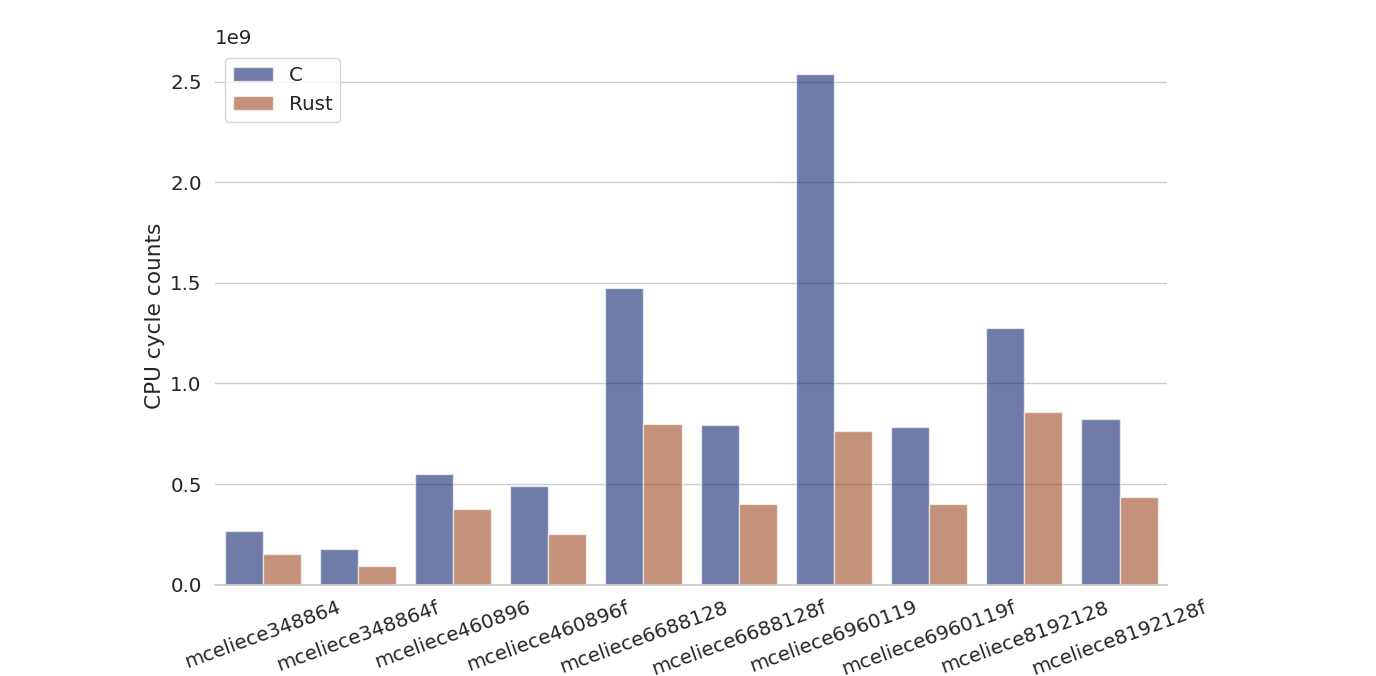
\includegraphics[width=1\textwidth]{images/completeKEM.png}
  \caption{Comparison between the CPU cycles of the Rust vs C implementation of the complete KEM operation.}
  \label{fig:plot1}
\end{figure}

\begin{figure}[H]
\centering
  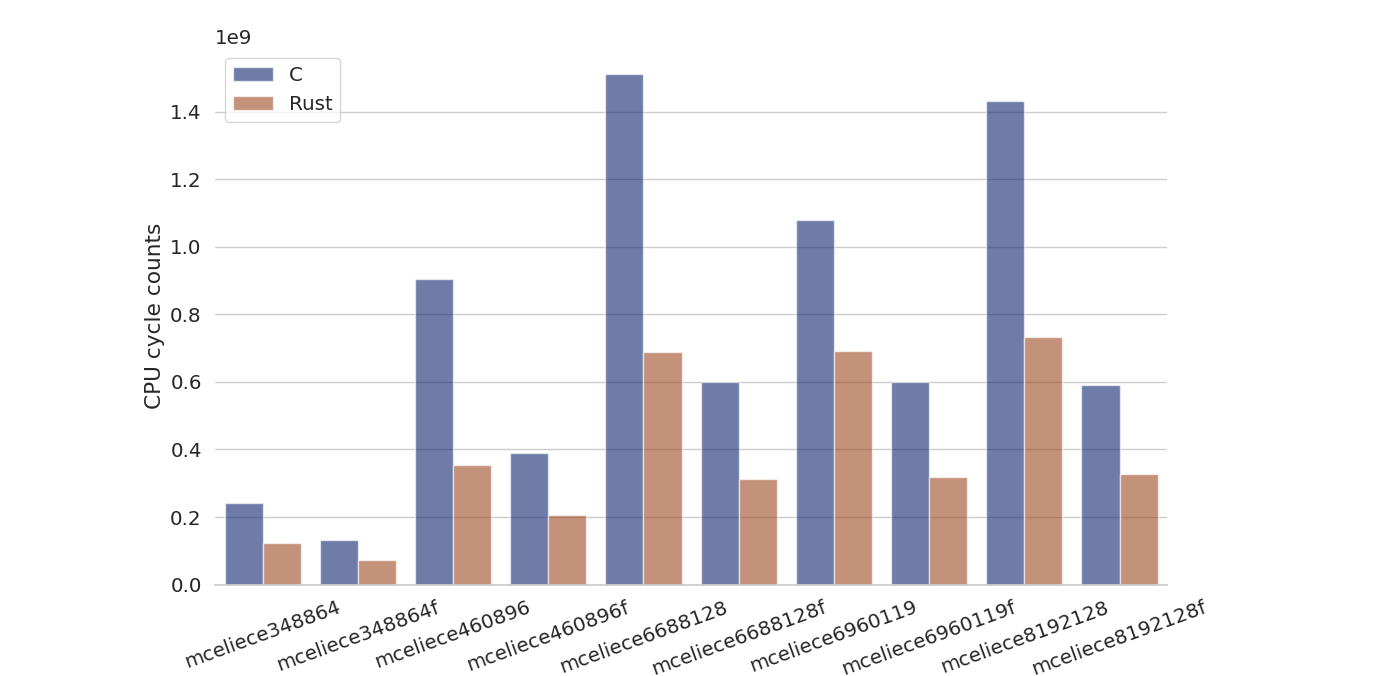
\includegraphics[width=1\textwidth]{images/keypair.png}
  \caption{Comparison between the CPU cycles of the Rust vs C implementation of the keypair subroutine.}
  \label{fig:plot1}
\end{figure}

\begin{figure}[H]
\centering
  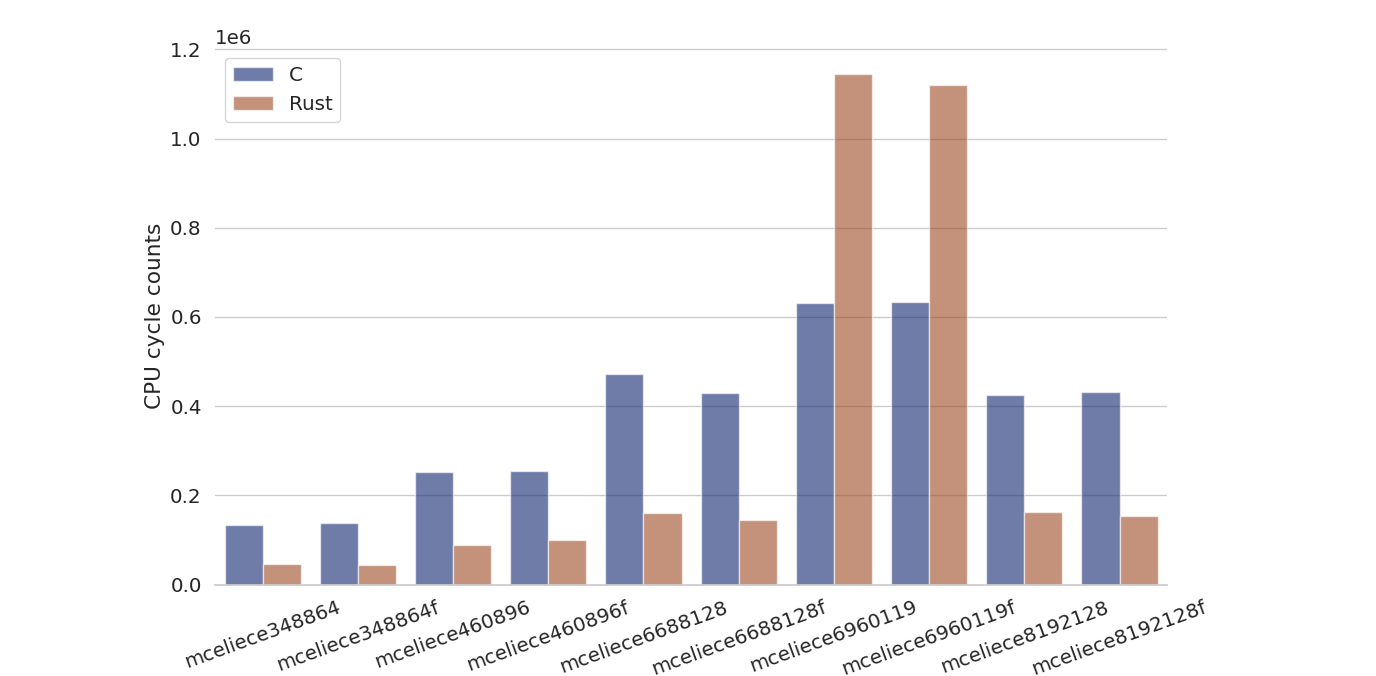
\includegraphics[width=1\textwidth]{images/encapsulation.png}
  \caption{Comparison between the CPU cycles of the Rust vs C implementation of the encapsulate subroutine.}
  \label{fig:plot1}
\end{figure}

\begin{figure}[H]
\centering
  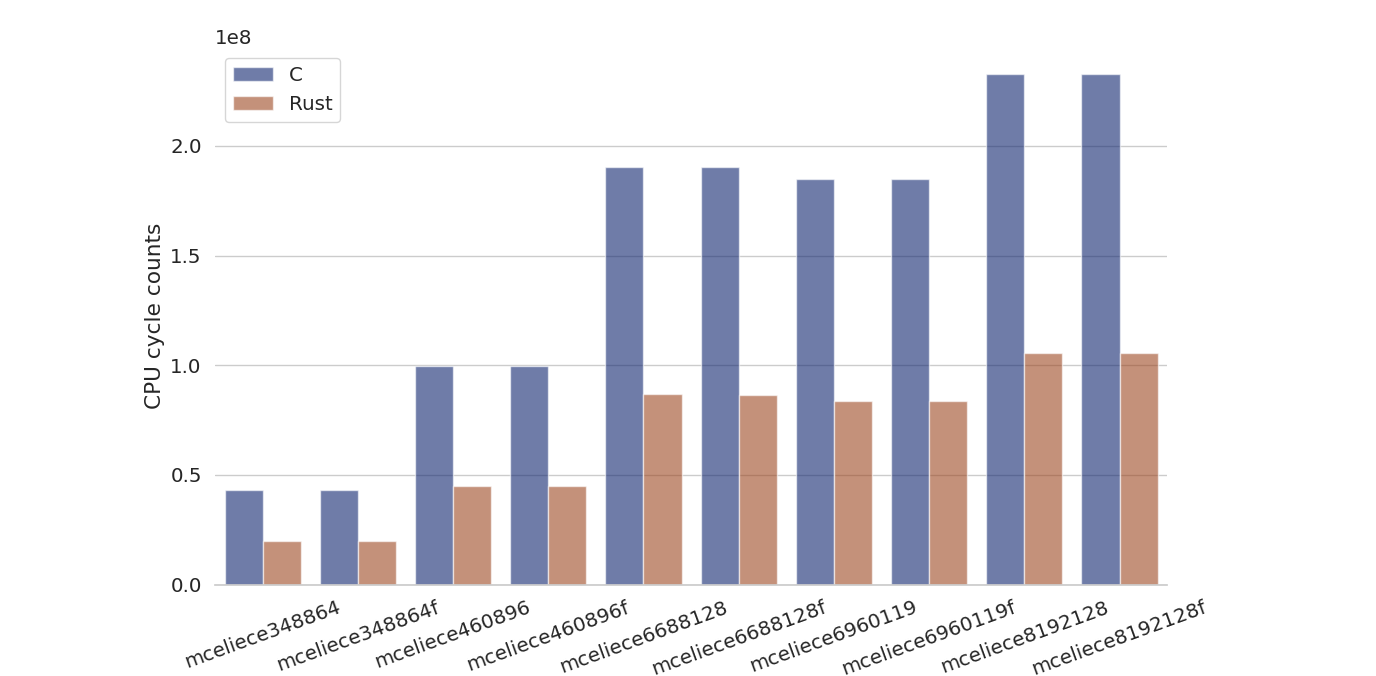
\includegraphics[width=1\textwidth]{images/decapsulation.png}
  \caption{Comparison between the CPU cycles of the Rust vs C implementation of the decapsulation subroutine.}
  \label{fig:plot1}
\end{figure}

\chapter{Conclusion}
\label{chap:conclusion}

The NIST reference implementation Classic McEliece was ported from the C language to the Rust programming language. When comparing Rust vs. C in benchmark scenarios, Rust ran faster than C in most experiments. A significant obstruction in the implementation was carefully paying attention to the used pointer arithmetic, array sizes, and type conversions to re-write these in the Rust language, which does not support raw-pointer manipulations, but instead relies on memory safety design features such as the described ownership model. Additional improvements of the implementation include refactoring the \inlinecode{layer\_ex} function as described in the evaluation part, refactoring for/while loops into, e.g., \inlinecode{clone\_from\_slice} function calls in order to achieve a more abstract code representation. Consequently, the compiler would be able to employ automatic vectorization or loop unrolling techniques to further optimize code execution. Furthermore, a more in-depth understanding of the post-quantum McEliece cryptosystem could be achieved by studying the background theory, dissecting the individual KEM algorithm subroutine calls and carefully inspecting them.


\chapter*{Acknowledgement}
\label{chap:acknowledgement}

First, I want to thank Lukas Prokop for introducing me to the thesis topic of writing Classic McEliece in Rust. I am thankful for the fruitful discussions concerning low-level bit manipulations, recursive matrix transpose implementations, and giving me a lot of advice in the Rust programming language.
Secondly, thank you, Daniel Kales for the thesis supervision takeover, reviewing my written thesis, and advising me on what could be improved. As my journey in the Software Engineering \& Management Bachelor program approaches its end, I want to embrace and thank all the friends I have made during this time. Thank's for working \& laughing together Johannes, Lena, Marcel, Ferdi, Mick, Flo, Alex, Markus, Steini, Kati, Dominik, Steffl, Thomas, Mario and I hope we keep in touch from time to time :-) I embrace the trip to the 36c3 ! I want to thank my family for supporting me and showing understanding and patience during intense study times.

%--- INDEX and BIBLIOGRAPHY ----------------------------------------------------

%% Print List of Acronyms and Symbols  (optional)
%\printnoidxglossary[title={Notation}]
%\printnoidxglossary[type=acronym]

% Print bibliography and include it in the table of contents:
\printbibliography[heading=bibintoc]

\end{document}
